\documentclass[12pt, a4 paper]{article}
\usepackage{babel}
\usepackage{graphicx, hyperref, xcolor, fancyhdr, amssymb, amsmath, amsthm}
\usepackage{mathrsfs}
\usepackage[acronym, toc]{glossaries}
\usepackage{pdfpages}
\usepackage{svg}
\usepackage{algorithmic}
\usepackage[ruled, linesnumbered]{algorithm2e}


% \usepackage{times}

\hypersetup{
    colorlinks,
    linkcolor={red!60!black},
    citecolor={blue!80!black},
    urlcolor={blue!80!black}
}

% \pagestyle{fancy}
% \renewcommand\headrulewidth{.5pt}
% \fancyhead[L]{
%     V. Trélat
% }

% \fancyhead[C]{
%     \textbf{Verification in Isabelle/HOL of Hopcroft's algorithm for minimizing DFAs including runtime analysis}
% }

% \fancyhead[R]{
%     % Current section
%     \ifnum\c@secnumdepth>0
%         \thesection
% }

% theorems
\newtheorem{theorem}{Theorem}
\newtheorem{lemma}{Lemma}
\newtheorem{remark}{Remark}

\theoremstyle{definition}
\newtheorem{definition}{Definition}

% Glossary

\makeglossaries

% \newacronym{tiaa}{TIAA}{This Is An Acronym}

\begin{document}

\begin{titlepage}
    \begin{center}
        \vfill
        
\includegraphics[height=1.5cm]{img/logoTUM.png}
        \hfill
        
\includegraphics[height=1.5cm]{img/logoartem.png}
        \hfill
        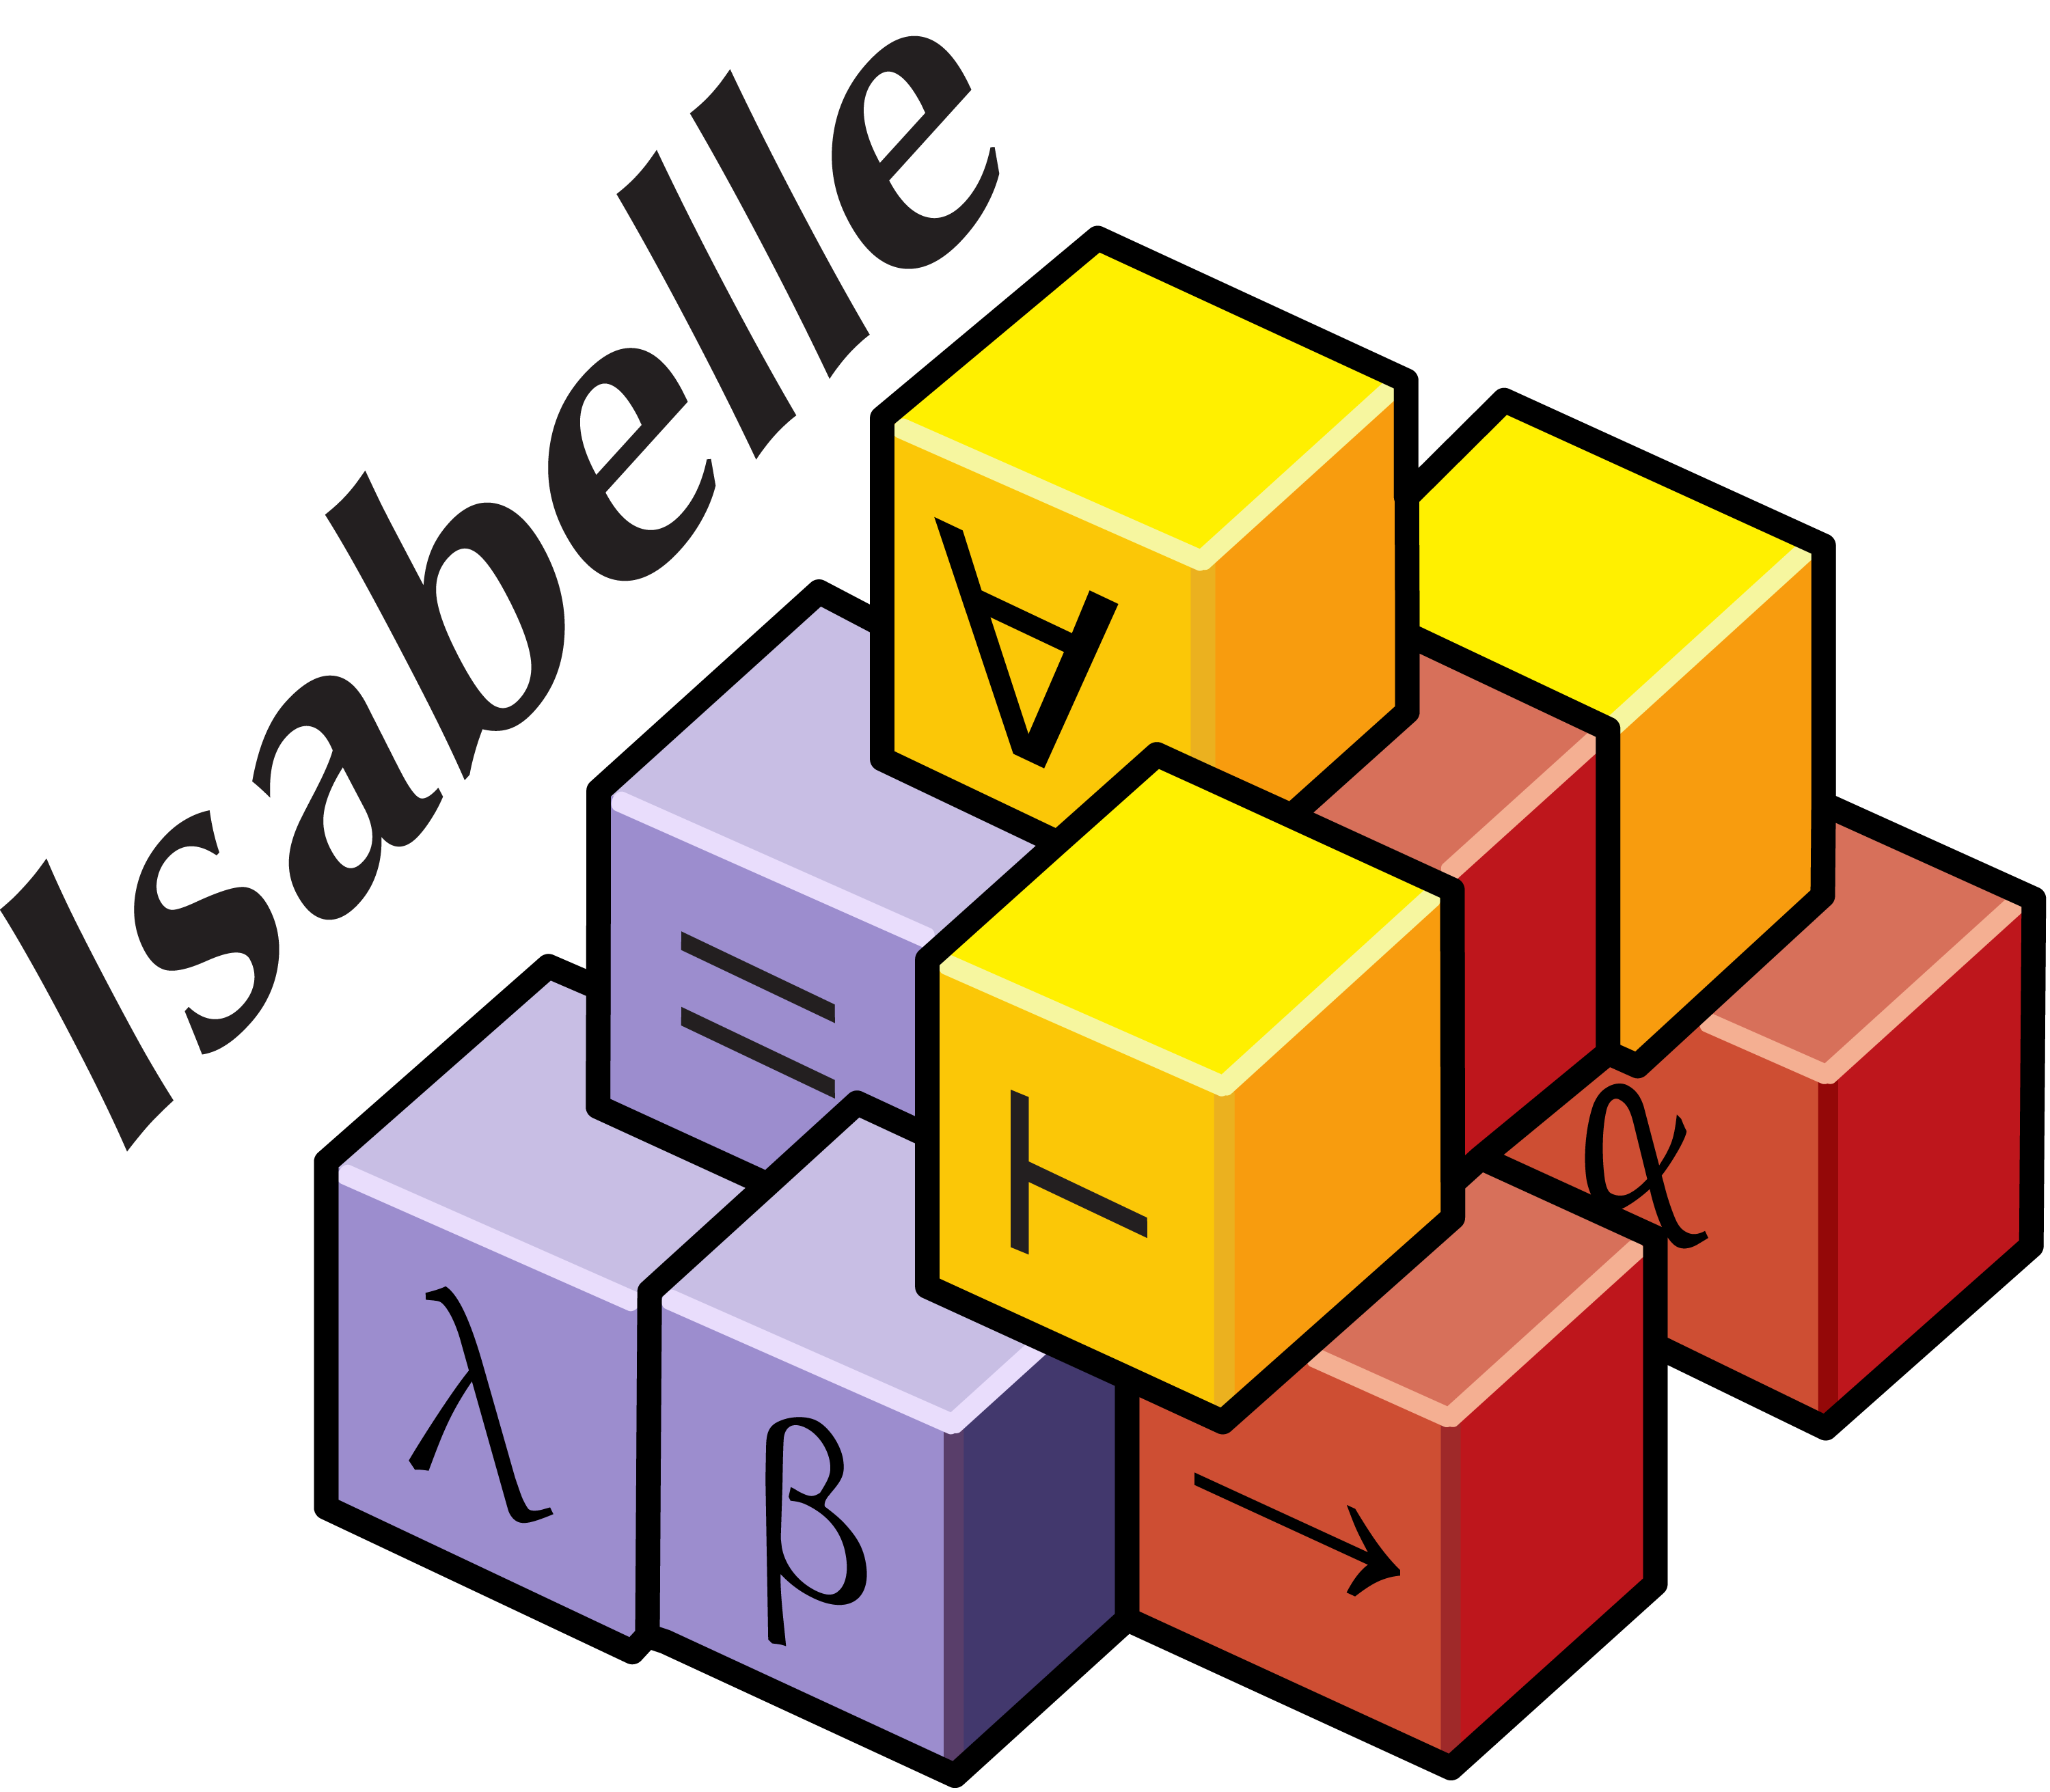
\includegraphics[height=1.5cm]{img/logoisabelle.png}
        \vfill
    \end{center}
    \begin{center}
        
        \textbf{Final year intership report}
        \vfill

        \large{\textbf{Verification in Isabelle/HOL of Hopcroft's algorithm for minimizing DFAs including runtime analysis}}
    \end{center}
    
    \vfill
    
    \begin{center}
        \textbf{Vincent Trélat}\\
        \vspace{1cm}
        \textit{\today}
    \end{center}
    \vfill
    \begin{center}
        
\includegraphics[height=1.2cm]{img/logoGE.png}
        \hfill
        
\includegraphics[height=1.2cm]{img/logoUL.png}
    \end{center}
\end{titlepage}

\tableofcontents

\pagebreak

\section{Introduction}
\subsection{Original algorithm}
John E. Hopcroft's algorithm for minimizing DFAs was first presented in his original 1971 paper \cite{Hop71} as a formal algorithm. Algorithm~\ref{alg:original} is a direct translation of the original algorithm with only slight changes in the notations.

\begin{algorithm}[H]
\SetAlgoLined
\caption{Hopcroft's original formal algorithm}
\label{alg:original}
\KwData{\textbf{Input:} a finite DFA $\mathcal{A} = (\mathcal{Q}, \Sigma, \delta, q_0, \mathcal{F})$}
\KwResult{\textbf{Output:} the equivalence class of $\mathcal{Q}$ under state equivalence}
Construct $\delta^{-1}(q, a) := \{t \in \mathcal{Q}\ |\ \delta(t, a) = q\}$ for all $q \in \mathcal{Q}$ and $a \in \Sigma$ \;\label{alg:original:1}
Construct $P_1 := \mathcal{F}$, $P_2 := \mathcal{Q} \setminus \mathcal{F}$ and $a_i := \{q \in P_i \ | \ \delta^{-1}(q, a) \neq \varnothing \}$ for all $i \in \{1, 2\}$ and $a \in \Sigma$ \;
Let $k := 3$ \;
For all $a \in \Sigma$, construct $L_a := \underset{0 \leq i < k}{\operatorname*{arg\,min}}\ \left| a_i \right|$ \; \label{alg:original:4}
\While{$\exists a \in \Sigma, L_a \neq \varnothing$}{
    Pick $a \in \Sigma$ such that $L_a \neq \varnothing$ and $i \in L_a$ \;
    $L_a := L_a \setminus \{i\}$ \;
    \ForAll{$j < k, \exists q \in P_j, \delta(q, a) \in a_i$}{
        $P'_j := \{t \in \mathcal{Q}\ |\ \delta(t, a) \in a_i \}$ and $P''_j := P_j \setminus P'_j$ \;
        $P_j := P'_j$ and $P_{k} := P''_j$; construct $a_j$ and $a_k$ for all $a \in \Sigma$ accordingly \;
        For all $a \in \Sigma$, $L_a := \begin{cases}
        L_a \cup \{j\} & \text{if $j \notin L_a \land \left| a_j \right| \leq \left| a_k \right|$} \\
        L_a \cup \{k\} & \text{otherwise}
        \end{cases}$ \;
        $k := k + 1$ \;
    }
}
\end{algorithm}

\subsection{Modern formalisation}

Today, the algorithm is usually given in a more mathematical and formalised way\footnote{see for example \cite{esparza2023automata}}, as presented below in Algorithm~\ref{alg:modern}.

\begin{definition}
    Let $\mathcal{A} = (Q, \Sigma, \delta, q_0, I, F)$ be a DFA. Let $P$ be a partition of $Q$. Let $B \in P$ and $a \in \Sigma$. We say for $C \in P$ that
    $(a, C)$ splits $B$ if $$\exists q_1, q_2 \in B \quad \delta(q_1, a) \in C \land \delta(q_2, a) \notin C.$$
\end{definition}

If $(a, C)$ is a splitter of $B$, $P$ can be updated to $P \setminus \{B\} \cup \{B', B''\}$, where $$B' := \{q \in B \ | \ \delta(q, a) \in C\} \text{ and } B'' := B \setminus B'.$$

\begin{algorithm}[H]
\SetAlgoLined
\caption{Hopcroft's algorithm in a modern style}
\label{alg:modern}
\KwData{\textbf{Input:} a finite DFA $\mathcal{A} = (\mathcal{Q}, \Sigma, \delta, q_0, \mathcal{F})$}
\KwResult{\textbf{Output:} the language partition $P_\ell$}
\eIf{$\mathcal{F} = \varnothing \lor \mathcal{Q} \setminus \mathcal{F} = \varnothing$}{
    \Return $\mathcal{Q}$
}{
    $P := \{ \mathcal{F}, \mathcal{Q} \setminus \mathcal{F} \}$ \;
    $\mathcal{W} := \{ (a, \min \{ \mathcal{F}, \mathcal{Q} \setminus \mathcal{F}\}, a \in \Sigma \}$ \;
    \While{$\mathcal{W} \neq \varnothing$}{
        Pick $(a, B')$ from $\mathcal{W}$ \;
        \ForAll{$B \in P$}{
            Split $B$ with $(a, B')$ into $B_0$ and $B_1$ \;
            $P := (P \setminus \{B\}) \cup \{B_0, B_1\}$ \;
            \ForAll{$b \in \Sigma$}{
                \eIf{$(b, B \in \mathcal{W})$}{
                    $\mathcal{W} := (\mathcal{W} \setminus \{(b, B)\}) \cup \{(b, B_0), (b, B_1)\}$ \;
                }{
                    $\mathcal{W} := \mathcal{W} \cup \{(b, \min \{ B_0, B_1 \})\}$ \;
                }
            }
        }
    }
}

\end{algorithm}

\section{Proof of correctness}
\section{Time complexity analysis}

We focus on the original algorithm presented in Algorithm~\ref{alg:original} in order to work on the arguments given in \cite{Hop71}. The data structures used at that time were mostly linked lists, but let us rather give some requirements for the data structures instead of actual implementations. The goal is to show that the algorithm can be executed in $O(m \cdot n \log n)$ time, where $m$ is the number of symbols in the alphabet and $n$ is the number of states in the DFA.

The following requirements come directly from \cite{Hop71} and are specific to the algorithm presented in Algorithm~\ref{alg:original}.
\begin{itemize}
    \item[\bf REQ1] Sets such as $\delta^{-1}(q, a)$ and $L_a$ must be represented in a way that allows $O(1)$ time for addition and deletion in front position.
    \item[\bf REQ2] Vectors must be maintained to indicate whether a state is in a given set.
    \item[\bf REQ3] Sets such as $P_i$ must be represented in a way that allows $O(1)$ time for addition and deletion at any given position.
    \item[\bf REQ4] For a state $q$ in a set $P_i$ or $a_i$, its position must be determined in $O(1)$ time.
\end{itemize}

Lines \ref{alg:original:1} to \ref{alg:original:4} can be executed in $O(\left| \Sigma \right| \cdot \left| \mathcal{Q} \right|)$ time (for example with DFS for the inverse transition function).

% \printglossary[type=\acronymtype]

% \addcontentsline{toc}{section}{CV}
% \includepdf{cv.pdf}

\pagebreak
% bibliography
\bibliographystyle{alpha}
\bibliography{ref}

\end{document}